\begin{frame}
\frametitle{Внешние устройства}
\begin{itemize}
  \item Допустим у вас есть сетевая карта:
  \begin{itemize}
    \item можно передать сетевой карте набор байт для отправки;
    \item сетевая карта может получать данные, процессор должен скопировать эти
    данные в память, обработать и "показать" пользователю;
    \item пакеты могут приходить в произвольные моменты времени;
  \end{itemize}
  \item как узнать, что данные пришли на сетевую карту?
  \begin{itemize}
    \item можно спросить устройство (проверить какой-нибудь бит в каком-нибудь
    регистре устройства);
    \item такой вариант называют \emph{polling};
    \item пока код исполняемый процессором опрашивает устройство, процессор не
    делает ничего полезного;
  \end{itemize}
\end{itemize}
\end{frame}

\begin{frame}
\frametitle{Прерывания}
\begin{itemize}
  \item Прерывания - сигнал процессору, который "прерывает" текущий исполняемый
  код процессора
  \begin{itemize}
    \item сетевая карта посылает сигнал при получении данных;
    \item вместо исполняемого кода вызывается специальный обработчик прерывания;
    \item обработчик прерывания обслуживает устройство, и возвращает управление
    прерванному коду.
  \end{itemize}
  \item Следствия:
  \begin{itemize}
    \item не нужно тратить ресурсы процессора на бесполезный опрос устройств;
    \item прерванный код может быть не готов к тому, что его прервут - задача
    обработчика позаботится об этом;
  \end{itemize}
\end{itemize}
\end{frame}

\begin{frame}
\frametitle{Контроллер прерываний}
\begin{itemize}
  \item А что если у нас много устройств требующих внимания процессора?
  \begin{itemize}
    \item какое из устройств сгенерировало прерывание?
    \item если сразу несколько устройств сгенерировали прерывания?
  \end{itemize}
  \item Для разрешения этих проблем нужен посредник между устройствами и
  процессором
  \begin{itemize}
    \item такого посрденика называют контроллером прерываний;
    \item контроллер прерываний выполняет арбитраж;
  \end{itemize}
\end{itemize}
\end{frame}

\begin{frame}
\frametitle{Intel 8259}
\begin{columns}
  \begin{column}{0.7\textwidth}
  Intel 8259 - \emph{программируемый} контроллер прерываний (далее просто PIC)
  \begin{itemize}
    \item каскад из двух PIC использовался в IBM PC начиная с AT;
    \item сейчас он не используется, но его поведение эмулируется современными
    контроллерами прерываний;
  \end{itemize}
  \end{column}
  \begin{column}{0.3\textwidth}
    \begin{center}
      \includegraphics[width=\textwidth]{i8259.jpg}
    \end{center}
  \end{column}
\end{columns}
\end{frame}

\begin{frame}
\frametitle{Каскад intel 8259}
\begin{columns}
  \begin{column}{0.5\textwidth}
  \begin{center}
    \includegraphics[height=0.7\textheight]{pic_cascade.png}
  \end{center}
  \end{column}
  \begin{column}{0.5\textwidth}
  \begin{itemize}
    \item 2 контроллера по 8 выходов - 1 выход = 15 внешних устройств;
    \item большинство из выходов в IBM PC заняты фиксировнными устройствами;
    \item вы тесно познакомитесь с PIT (programmable interval timer);
  \end{itemize}
  \end{column}
\end{columns}
\end{frame}

\begin{frame}
\frametitle{Обработка прерываний}
\begin{itemize}
  \item Чтобы получать и обрабатывать прерывания необходимо:
  \begin{itemize}
    \item запрограммировать контроллер прерываний (PIC);
    \item указать процессору, где находятся обработчики прерываний;
  \end{itemize}
  \item на x86 для указания на обработчики прерываний используется IDT
  \begin{itemize}
    \item IDT (interrupt descriptor table) - таблица из максимум 256
    дескрипторов, описывающих обработчики прерывания;
    \item т. е. в x86 архитектуре можно задать не более 256 обработчиков
    прерываний;
    \item из них первые 32 зарезервированы, т. е. остается 224 под наши нужды;
  \end{itemize}
\end{itemize}
\end{frame}

\begin{frame}
\frametitle{IDT}
\begin{center}
  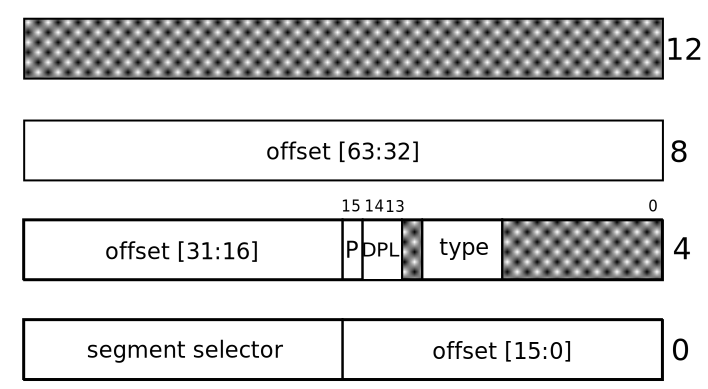
\includegraphics[width=0.5\textwidth]{idt.png}
\end{center}
\begin{itemize}
  \item \emph{offset} - адрес обработчика;
  \item \emph{segment selector} - селектор (регистр CS);
  \item \emph{P} (Present) - должен быть равен 1;
  \item \emph{type} - домашнее задание разобраться в разнице между Interrup
  Gate и Trap Gate;
  \item все остальное должно быть равно 0;
\end{itemize}
\end{frame}

\begin{frame}
\frametitle{IDTR}
\begin{center}
  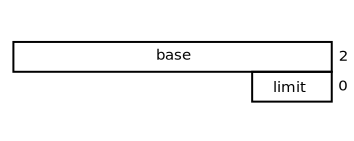
\includegraphics[width=0.6\textwidth]{idt_ptr.png}
\end{center}
\begin{itemize}
  \item Информация о местоположении IDT хранится в специальном регистре (IDTR);
  \item загрузить значение в регистр можно с помощью специальной инструкции
  lidt;
  \begin{itemize}
    \item параметром инструкции является специальный "дескриптор";
    \item \emph{base} - 64-битный адрес IDT в памяти;
    \item \emph{limit} - 16-битный размер IDT в байтах минус единица;
  \end{itemize}
\end{itemize}
\end{frame}

\begin{frame}
\frametitle{Программирование PIC}
\begin{itemize}
  \item Как выбирается какую запись IDT использовать при прерывании?
  \begin{itemize}
    \item вам нужно записать в контроллер на какие записи IDT отображаются
    входы контроллера;
    \item в случае PIC, вам нужно указать на какую запись IDT отображается
    самый первый вход каждого контроллера, все остальные идут по порядку.
  \end{itemize}
  \item Кроме отображения контроллеру прерываний также нужно указать:
  \begin{itemize}
    \item конфигурацию каскада (как Master и Slave соединены);
    \item тип прерывания (edge/level);
    \item и много другого не интересного;
  \end{itemize}
\end{itemize}
\end{frame}

\begin{frame}
\frametitle{Взаимодействие с PIC}
\begin{itemize}
  \item Для общения с PIC используются два 8-ми битных регистра: регистр команд
  и регистр данных;
  \begin{itemize}
    \item в регистр команд записывается действие, которое нужно сделать;
    \item затем в регистр данных записываются данные (сколько и какие именно
    зависит от команды).
  \end{itemize}
  \item Для доступа к регистрам PIC-ов в x86 используется пространство
  ввода/вывода и специальные инструкции работы с ним:
  \begin{itemize}
    \item инструкции называются \emph{in} и \emph{out}, а аргументы порт
    ввода/вывода и данные;
    \item регистр команд Master PIC соответствует порту \emph{0x20}, а регистр
    данных порту \emph{0x21};
    \item Slave PIC использует порты \emph{0xA0} и \emph{0xA1};
  \end{itemize}
\end{itemize}
\end{frame}

\begin{frame}
\frametitle{Отображение входов PIC}
\begin{itemize}
  \item Чтобы настроить отображение необходимо записать в командный регистр
  значение \emph{0x11} - команда инициализации контроллера;
  \item команда инициализации ожидает три байта данных:
  \begin{itemize}
    \item номер записи IDT, соответвующей самой первому входу контроллера;
    \item параметры каскада:
    \begin{itemize}
      \item для Master PIC - битовую маску входов, к котороым подключены Slave
      PIC-и (в нашем случае это просто \emph{4} - 2-ой бит равен 1, остальные
      0);
      \item для Slave PIC - номер входа Master PIC, к которому он подключен (в
      нашем случае это 2);
    \end{itemize}
    \item прочие неинтересные параметры (в нашем случае нужно записать число
    \emph{1});
  \end{itemize}
\end{itemize}
\end{frame}

\begin{frame}
\frametitle{Маскировка прерываний}
\begin{itemize}
  \item Иногда полезно запретить доставку определенных прерываний
  (замаскировать)
  \begin{itemize}
    \item до того как драйвер/ОС настроило устройство, прерывания от него лучше
    отключить;
    \item т. е. пре инициализации PIC все прерывания лучше замаскировать;
  \end{itemize}
  \item Для маскировки прерываний в случае PIC используется регистр данных:
  \begin{itemize}
    \item запишите в регистр данных битовую маску прерываний (замаскированным
    соответсвуют 1-цы);
    \item обратите внимание, что писать что-либо в командный регистр не нужно;
  \end{itemize}
\end{itemize}
\end{frame}
